% Copyright (c)  2005-2010 EDF-EADS-PHIMECA.
% Permission is granted to copy, distribute and/or modify this document
% under the terms of the GNU Free Documentation License, Version 1.2
% or any later version published by the Free Software Foundation;
% with no Invariant Sections, no Front-Cover Texts, and no Back-Cover
% Texts.  A copy of the license is included in the section entitled "GNU
% Free Documentation License".
\renewcommand{\filename}{docUC_InputWithData_FittingTests.tex}
\renewcommand{\filetitle}{UC : Distribution fitting tests, numerical and visual validation tests : Chi-squared test, Kolmogorov test, QQ-plot graph}

% \HeaderNNIILevel
% \HeaderIILevel
\HeaderIIILevel



\index{Graph!QQ-plot}
\index{Graph Manipulation!Bounding box}
\index{Graph Manipulation!ViewImage}
\index{Graph Manipulation!Show}
\index{Fitting Test!QQ-plot}
\index{Fitting Test!ChiSquared}
\index{Fitting Test!Kolmogorov}
\index{Fitting Distribution!Parametric method}



The objective of this Use Case is to :
\begin{itemize}
\item perform some parametric fitting tests on a numerical sample in dimension 1, with the maximum likelihood principle or the moment based method,
\item validate these estimations with numerical tests : the Kolmogorov test (continuous distributions) or the Chi -squared test (discrete distributions),
\item validate these estimations with a visual test : the QQ-plot graph.
\end{itemize}

The QQ-plot visual validation test is used with a numerical sample (representing the data) and a distribution (representing the fitted one). For each point of the numerical sample used in the graph, Open Turns evaluates its empirical quantile and associates to it the corresponding quantile from the fitted distribution. \\

Details on the Maximum Likelihood  Principle may be found in the Reference Guide (\href{OpenTURNS_ReferenceGuide.pdf}{see files Reference Guide - Step B -- Maximum Likelihood  Principle}).\\

Details on the Parametric estimators used to evaluate the parameters of the copula may be found in the Reference Guide (\href{OpenTURNS_ReferenceGuide.pdf}{see files Reference Guide - Step B --  Parametric Estimation}).\\

Details on the QQ-polt, Kolmogorov-Smirnov and  Chi-squared tests may be found in the Reference Guide (\href{OpenTURNS_ReferenceGuide.pdf}{see files Reference Guide - Step B --  Graphical goodness-of-fit tests : QQ-plot and Henry line and Step B -- Kolmogorov-Smirnov goodness-of-fit test}).\\

Details on each object may be found in the User Manual  (\href{OpenTURNS_UserManual_TUI.pdf}{see User Manual - Statistics on sample /  Distribution factory and /Fitting test}).\\



The example here presents :
\begin{itemize}
\item the fitting of a numerical sample of dimension 1 with a Beta distribution, its validation with the Kolmogorov test and the  QQ-Plot graph,
\item the fitting of a numerical sample of dimension 1 with a Poisson distribution, its validation with the Chi-squared test and the  QQ-Plot graph.
\end{itemize}


\requirements{
  \begin{description}
  \item[$\bullet$] a scalar numerical sample (data) : {\itshape sample}
  \item[type:]  NumericalSample
  \end{description}
}
{
  \begin{description}
  \item[$\bullet$] a Beta fitted continuous distribution : {\itshape estimatedBetaDistribution}
  \item[type:] Beta
  \item[$\bullet$] a Uniform continuous fitted distribution : {\itshape estimatedUniformDistribution}
  \item[type:] Uniform
  \item[$\bullet$] a Poisson discrete fitted distribution : {\itshape estimatedPoissonDistribution}
  \item[type:] Poisson
  \item[$\bullet$] the files containing the QQ-plot graph : {\itshape QQPlot.png, QQPlot.eps}
  \item[type:] files at format PNG or EPS or FIG
  \item[$\bullet$] a numerical validation by the Kolmogorov test for two continuous distributions (p-value)
  \item[type:] TestResult
  \item[$\bullet$] a numerical validation by the Chi-squared test for  discrete distribution (p-value)
  \item[type:] TestResult
  \end{description}
}

\textspace\\
Python script for this UseCase :

\begin{lstlisting}
  # Fit a Beta distribution to the sample
  # Create a Beta factory
  factory = BetaFactory()

  # Estimate the beta parameters
  # We estimate all the parameters of the Beta distribution from sample
  estimatedBetaDistribution = factory.build(sample)

  # Get the parameters of the estimated distribution
  estimatedParam = estimatedBetaDistribution.getParameters()

  # Display the resulted distribution with its parameters
  print "Estimated Beta distribution=", estimatedBetaDistribution

  # Validate the Beta fitted distribution with the Kolmogorov Test
  # Test = True <=> the sample follows a Beta distribution (H0 hypothesis)
  # p-value threshold : probability of the H0 reject zone = 1-0.95
  # p-value : probability (test variable decision > test variable decision evaluated on the samples)
  # Test = True (=1) <=> p-value > p-value threshold
  resultKolmogorov =  FittingTest.Kolmogorov(sample, Distribution(estimatedBetaDistribution), 0.95)

  # Print result of the Kolmogorov Test
  print "Test Succes ? ", (resultKolmogorov.getBinaryQualityMeasure()==1)

  # Get the p-value of the Kolmogorov Test
  print "p-value of the Kolmogorov Test = ", resultKolmogorov.getPValue()

  # Get the p-value threshold of the Kolmogorov Test
  print "p-value threshold = ", resultKolmogorov.getThreshold()

  # Validate the Beta fitting with a visual test : QQ-plot test
  # Generate the Graph structure for the QQ-plot graph
  # number of points of the graph fixed to 100 (20 by default)
  sampleBetaQQPlot = VisualTest.DrawQQplot(sample, estimatedBetaDistribution, 100)

  # Impose a bounding box : x-range and y-range
  # boundingBox = [xmin, xmax, ymin, ymax]
  myBoundingBox = NumericalPoint( (xmin, xmax, ymin, ymax) )
  sampleBetaQQPlot.setBoundingBox(myBoundingBox)

  # In order to extract the QQ-plot line
  myCurve = sampleBetaQQPlot.getDrawable(1)

  # In order to see the graph without creating the associated files
  Show(sampleBetaQQPlot)

  # Draw the graph on the file BetaQQPlot.png and twoSamplesQQPlot.eps
  # if the file adress is not fulfilled, the file is created in the current directory
  sampleBetaQQPlot.draw("SampleBetaQQPlot")

  # View the bitmap file
  ViewImage(sampleBetaQQPlot.getBitmap())

  # Check if it worked
  print "bitmap = ", sampleBetaQQPlot.getBitmap()
  print "postscript = ", sampleBetaQQPlot.getPostscript()

  # Fit a Poisson distribution to the sample
  # Create a Poisson factory
  factory = PoissonFactory()

  # Estimate the Poisson parameters
  # We estimate all the parameters of the Poisson distribution from sample
  estimatedPoissonDistribution = factory.build(sample)

  # Display the resulted distribution with its parameters
  print "Estimated Poisson distribution=", estimatedPoissonDistribution

  # Validate the Poisson fitted distribution with the Chi-squared Test
  # Test = True <=> the sample follows a Beta distribution (H0 hypothesis)
  # p-value threshold : probability of the H0 reject zone = 1-0.95
  # p-value : probability (test variable decision > test variable decision evaluated on the samples)
  # Test = True (=1) <=> p-value > p-value threshold
  # Number of parameters estimated from sample : 1
  resultChiSquared =  FittingTest.ChiSquared(sample, estimatedPoissonDistribution, 0.95, 1)

  # Print result of the Chi-squared Test
  print "Test Succes ? ", (resultChiSquared.getBinaryQualityMeasure()==1)

  # Get the p-value threshold of the Chi-squared Test
  print "p-value threshold = ", resultChiSquared.getPValue()

  # Get the p-value threshold (corresponding to the confidence level) of the Chi-squared Test
  print "p-value of the Chi-squared Test = ", resultChiSquared.getThreshold()
\end{lstlisting}
\textspace\\


Figures \ref{qqplotExRight} and \ref{qqplotExFalse} show a QQ-Plot graph to test the adequation of a sample coming from a Beta(r = 1.2, t = 3.4, a = 1.0, b = 2.0) to :
\begin{itemize}
\item the Beta(r = 1.2, t = 3.4, a = 1.0, b = 2.0) distribution : visual validation of the fitting,
\item the Weibull($\mu$ = 1.5, $\sigma$ = 1.0, $\gamma$ = 1.0) : visual invalidation of the fitting.
\end{itemize}




\begin{figure}[H]
  \begin{center}
    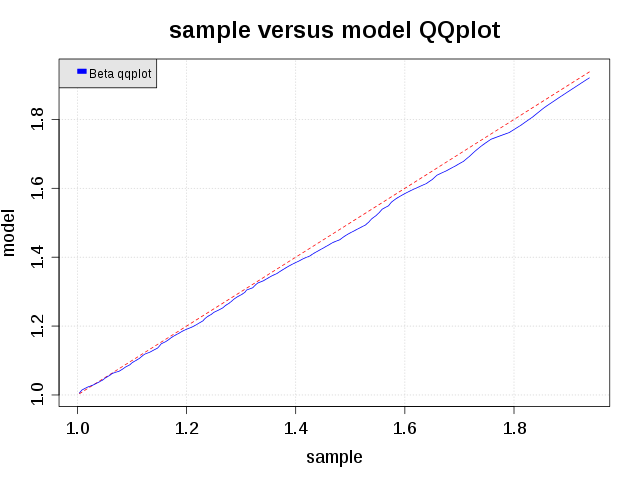
\includegraphics[width=10cm]{beta_QQplot.png}
  \end{center}
  \caption{Fitting validation by the QQ-Plot graph : Beta fitting to a Beta-sample.}
  \label{qqplotExRight}
\end{figure}

\begin{figure}[H]
  \begin{center}
    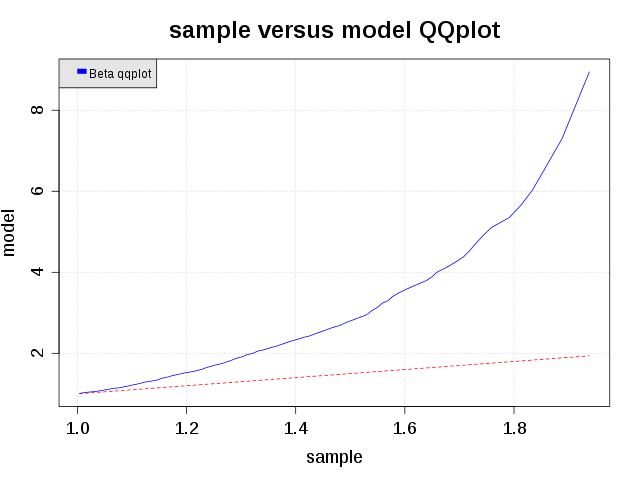
\includegraphics[width=10cm]{weibull_QQplot.png}
  \end{center}
  \caption{Fitting invalidation by the QQ-Plot graph : Weibull fitting to a Beta sample.}
  \label{qqplotExFalse}
\end{figure}

